
%(BEGIN_QUESTION)
% Copyright 2012, Tony R. Kuphaldt, released under the Creative Commons Attribution License (v 1.0)
% This means you may do almost anything with this work of mine, so long as you give me proper credit

Trefase asynkronmotorer reagerer ulikt på fasesvikt avhengig av om de er internt Y- eller delta-koblet:

$$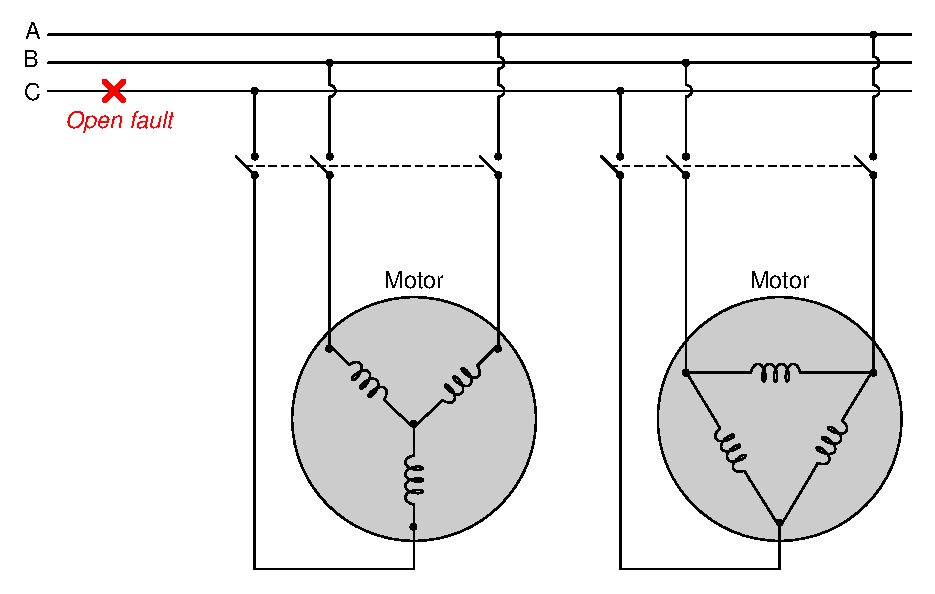
\includegraphics[width=15.5cm]{i00967x01.eps}$$

Hvilken motortype tåler fasesvikt best, og hvorfor?

\underbar{file i00967}
%(END_QUESTION)





%(BEGIN_ANSWER)

Delta-koblet motor tåler dette best, fordi den fortsatt danner et roterende flerfasefelt, mens Y-koblet motor i større grad får oscillerende felt. Hver fasevikling i delta beholder også full linjespenning.

Ved lett mekanisk last kan begge fortsette å rotere, men delta-koblet har større momentkapasitet i fasesvikt.

%(END_ANSWER)





%(BEGIN_NOTES)


%INDEX% Electronics review: 3-phase voltage/current/power calculation

%(END_NOTES)

